%========================================================================================
% Compilation should work with PDFLaTeX
%========================================================================================
% Type of document and general formatting
\documentclass[a4paper,11pt]{article}

\usepackage[left=2.5cm,right=2.5cm,top=2.5cm,bottom=2.5cm]{geometry}
\linespread{1.25}

%========================================================================================
% These packages are for language and font settings
\usepackage[english,activeacute]{babel} % Language
\usepackage{tgpagella}					% Text font
\usepackage[T1]{fontenc}				% T1 Encoding of font
\usepackage[utf8]{inputenc}				% Special symbols
\usepackage{lmodern}


%========================================================================================
\usepackage[sc]{mathpazo}				% Math font
\usepackage{amsmath,amsfonts,amssymb}	% Math symbols
\usepackage{dsfont}						% Math symbols like R for reals...
\usepackage{amsthm}						% For theorem styles
\usepackage{siunitx}

%========================================================================================
% Other packages
\usepackage{graphicx}
\usepackage{longtable}
\usepackage[svgnames]{xcolor}

%========================================================================================
\usepackage{accents}
\newcommand*{\dt}[1]{%
	\accentset{\mbox{\large\bfseries .}}{#1}} % Larger dot for time derivative


\usepackage{hyperref}
\hypersetup
{
    pdfauthor={Rafael Serrano-Quintero},
    pdfsubject={SIR Notes},
    colorlinks = {true},
    linkcolor = {FireBrick},
    citecolor = {FireBrick},
    urlcolor = {RoyalBlue},
}

\usepackage{appendix}
\usepackage{marvosym}
\usepackage{enumerate} %For enumerating with letters with option [a)]
\usepackage{enumitem}
\usepackage{fancyvrb}  %To reduce font size in verbatim environment
\usepackage{epstopdf}
\usepackage[flushleft]{threeparttable}
\usepackage{pdflscape}
\usepackage{natbib}
\usepackage{subcaption}
\usepackage{booktabs}
\usepackage[super]{nth}
\usepackage{float}

\newcommand{\source}[1]{\caption*{\tiny Source: {#1}} }

% Avoid warning for textbullet font
\renewcommand\textbullet{\ensuremath{\bullet}}
%========================================================================================
% Stata Preamble for Tables
%========================================================================================

\newcommand{\sym}[1]{\rlap{#1}}% Thanks to David Carlisle

\let\estinput=\input% define a new input command so that we can still flatten the document

\newcommand{\estwide}[3]{
		\vspace{.75ex}{
			\begin{tabular*}
			{\textwidth}{@{\hskip\tabcolsep\extracolsep\fill}l*{#2}{#3}}
			\toprule
			\estinput{#1}
			\bottomrule
			\addlinespace[.75ex]
			\end{tabular*}
			}
		}	

\newcommand{\estauto}[3]{
		\vspace{.75ex}{
			\begin{tabular}{l*{#2}{#3}}
			\toprule
			\estinput{#1}
			\bottomrule
			\addlinespace[.75ex]
			\end{tabular}
			}
		}

% Allow line breaks with \\ in specialcells
	\newcommand{\specialcell}[2][c]{%
	\begin{tabular}[#1]{@{}c@{}}#2\end{tabular}}

% *****************************************************************
% Custom subcaptions
% *****************************************************************
% Note/Source/Text after Tables
\newcommand{\figtext}[1]{
	\vspace{-1.9ex}
	\captionsetup{justification=justified,font=footnotesize}
	\caption*{\hspace{6pt}\hangindent=1.5em #1}
	}
\newcommand{\fignote}[1]{\figtext{\emph{Note:~}~#1}}

\newcommand{\figsource}[1]{\figtext{\emph{Source:~}~#1}}

% Add significance note with \starnote
\newcommand{\starnote}{\figtext{* p < 0.1, ** p < 0.05, *** p < 0.01. Standard errors in parentheses.}}

% *****************************************************************
% siunitx
% *****************************************************************
\usepackage{siunitx} % centering in tables
	\sisetup{
		detect-mode,
		tight-spacing           = true,
		group-digits            = false ,
		input-signs             = ,
		input-symbols           = ( ) [ ] - + *,
		input-open-uncertainty  = ,
		input-close-uncertainty = ,
		table-align-text-post   = false
        }

% Document parameters
\title{SIR Notes}
\author{Rafael Serrano Quintero \\
Dpt. Fundamentos del An\'alisis Econ\'omico \\
University of Alicante}
\date{}

\theoremstyle{definition}
\newtheorem{definition}{Definition}
\newtheorem{property}{Property}
\newtheorem{example}{Example}
\newtheorem{remark}{Remark}
\theoremstyle{plain}
\newtheorem{theorem}{Theorem}
\newtheorem{lemma}{Lemma}

% Height of figures
\newlength{\twosubht}
\newsavebox{\twosubbox}

%========================================================================================
					% === Title, thanks, and author data === %
%========================================================================================

\begin{document}      

\maketitle

\section{Differential Equations and Pandemics}\label{differential-equations-and-pandemics}

\subsection{Susceptible, Infected, Recovered Model}\label{susceptible-infected-recovered-model}

Infectious diseases such as COVID-19 are transmitted from one person to another. The most basic framework to understand their evolution is to divide population \((N)\) into three separate groups. Susceptible people \((S(t))\) are those who do not currently have the disease and can get it, infected people \((I(t))\) are those who currently have the disease, and recovered people \((R(t))\) are people who already passed the disease and recovered from it (or passed away) and cannot get it again. The SIR model thus describes the dynamics of the three population groups jointly. Let us normalize population to \(1\) so that \(S(t)\) is the share of total population that is susceptible, this will simplify calculations.

Let us describe the dynamics of the simplest SIR model. The basic assumptions are

\begin{itemize}
	\item Fixed total population \(N\) at a constant number
	\item Constant rates of transmission, recovery\ldots{}
	\item Fully mixed population
\end{itemize}

The first two assumptions are easily modified by describing a slightly more complex model but we will not worry about this. The third assumption implies that the probability for any infected person to contact any susceptible individual is equal to the average.  Let's start by describing the dynamics for susceptible people, a person stops being susceptible only if she gets the infection. Thus, the growth rate of total susceptible population declines with the contact with the infected population. Therefore,

\[
\frac{\partial S(t)}{\partial t} = - \beta S(t)I(t)
\] 
where \(\beta\) is the effective contact rate or transmission rate. This parameter tells us how likely it is that the infection is transmitted from an infected to a susceptible individual on average.

The share of infected people can either increase because more susceptible become infected, or decline because people recover from the disease. The first part is simply the opposite of the evolution of susceptible individuals, the second part will determine the recovery rate. Thus, 
\[
\frac{\partial I(t)}{\partial t} = \beta S(t)I(t) - \gamma I(t)
\] 
where \(\gamma\) is the recovery rate or the rate at which infected people stop being infected. It is easy to see that the dynamics for the recovered people will be given by 
\[
\frac{\partial R(t)}{\partial t} = \gamma I(t)
\]

\subsection{Conditions for a Pandemic}\label{conditions-for-a-pandemic}
That a disease is infectious does not mean it becomes a pandemic. What
are the necessary conditions for a pandemic? For there to be a pandemic, the share of infected people needs to grow over time, therefore \(\frac{\partial I(t)}{\partial t} > 0\), this implies

\[ 
\beta S(t)I(t) - \gamma I(t) > 0 \Rightarrow \frac{\beta S(t)I(t)}{\gamma} > I(t)
\] 

When the epidemic is about to start, almost nobody has the disease yet, therefore, we could assume \(S(t) \approx 1\) and cancel out the \(I(t)\). This will give us
\[
\frac{\beta}{\gamma} = \mathcal{R}_0 > 1
\] 
which implies that the \(\mathcal{R}_0\) or basic reproduction number
needs to be larger than one. This implies that a single infected individual passes the infection to more than one person. Note that this
\textbf{basic} reproduction number needs a \textbf{fully susceptible
population}. The effective reproduction number will be given by \[
\mathcal{R}^e_0 = \frac{\beta}{\gamma}S(0)
\]

\subsection{Analysis in the Long-Run}\label{analysis-in-the-long-run}
Is the number of infected people well defined in this model in the
long-run (as time goes to infinity)? It turns out it is. Note first that the right-hand side of the law of motion for the susceptible is negative and positive for the recovered. This implies

\[ 
\frac{\partial S(t)}{\partial t} \leq 0 \ ; \ \frac{\partial R(t)}{\partial t} \geq 0
\] 

Furthermore, the population is fixed and

\[ 
0 \leq S(t) \leq S(0) \leq N \ ; \ 0 \leq R(0) \leq R(t) \leq N
\] 

Which further implies

\[
\lim_{t\rightarrow \infty} S(t) = S(\infty) \ ; \ \lim_{t\rightarrow \infty} R(t) = R(\infty)
\] 
are well defined. Since \(1 = S(t) + I(t) + R(t)\), \(I(t) = 1 - S(t) - R(t)\), therefore 

\[
\lim_{t\rightarrow\infty} I(t) = I(\infty) = 1 - S(\infty) - R(\infty)
\]

Can we determine how the infected population evolves as a function of the susceptible people only? Yes! Note that

\[
\frac{1}{S(t)}\frac{\partial S(t)}{\partial t} = \frac{\dot{S}(t)}{S(t)} = -\beta I(t)
\] dividing by the law of motion for recovered

\[
\frac{\dot{S}(t)}{S(t)} = -\frac{\beta}{\gamma}\dot{R}(t)
\]

This is a separable differential equation. Integrating with respect to
time on both sides from \(0\) to \(t\)

\[
\int_0^t \frac{1}{S(t)} dS = -\frac{\beta}{\gamma}\int^t_0 dR
\]

Integrating and rearranging \[
\log(S(t)/S(0)) = -\frac{\beta}{\gamma}(R(t) - R(0))
\]

As before, we can express \(I(t) = 1 - S(t) - R(t)\). Solving in
previous expression for \(R(t)\) and substituting, we get

\[
I(t) = 1 - S(t) - R(0) + \frac{\gamma}{\beta}\log(S(t)/S(0))
\]

\subsection{Does everyone become infected?}\label{does-everyone-become-infected}

Imagine this was the case, then we can use previous expression assuming \(S(\infty) = 0\). Then, \[
I(\infty) = -\infty \] or, basically, the amount of infected people goes to zero.
 Is this because we run out of people to infect? In fact, no, we have shown that \(I(\infty) = 0\) for some positive value \(S(\infty)\). Thus, the equation for the infected must be satisfied with
\(I(\infty) = 0\) for \(S(\infty) > 0\). Then  

\[
\log(S(\infty)) = \log(S(0)) - \frac{\beta}{\gamma}(1 - R(0) - S(\infty)) 
\]

For typical initial conditions \(S(0) \approx 1\) and \(R(0) = 0\), 
\[
\log(S(\infty)) = - \frac{\beta}{\gamma}(1 - S(\infty))
\]

\subsection{How do cases evolve?}\label{how-do-cases-evolve}
Recall we have defined our basic reproduction number as
\(\mathcal{R}_0 = \frac{\beta}{\gamma}\) but our \emph{effective} reproduction number as \(\mathcal{R}^e_0 = \frac{\beta}{\gamma} S(0)\). Using the law of motion for the infected people \[
\dot{I}(t) = \beta S(t)I(t) - \gamma I( ) = (\beta S(t) - \gamma)I(t) \] recalling that \(0 \leq S(t) \leq S(0) \leq 1\), we can say that \[ \dot{I}(t) = (\beta S(t) - \gamma)I(t) \leq (\beta S(0) - \gamma)I(t) = \gamma (\mathcal{R}^e_0 - 1)I(t)
\]  

There are two possibilities depending on the effective reproduction number. If it is below \(1\), then previous expression is lower or equal than  \(0\) and thus, the amount of infected people decreases monotonically to \(0\). If \(\mathcal{R}^e_0\) is larger than \(1\) we can look back to the law of motion for infected cases and ask at which level of susceptible people the growth rate of infected people is zero, that is

\[
\frac{\dot{I}}{I} = \beta S^* - \gamma = 0 \Rightarrow S^* = \frac{\gamma}{\beta} > 0
\]

Going to the formula for infected cases as a function of \(S(t)\), we
can see that the maximum number of infected people is

\[
I_{max} = 1 - R(0) - \frac{\gamma}{\beta}\left(1 - \log\left(S(0)\frac{\beta}{\gamma}\right)\right)
\]

Note that the maximum number of infected people depends on the initial conditions for $R(0)$ and $S(0)$. What this shows is that the more immune people to the disease at the beginning the lower the maximum number of infected people. In other words, herd-immunity helps controlling the pandemic.

\subsection{Quantitative Analysis of the Model}\label{quantitative-analysis-of-the-model}

We have shown several important features of infectious diseases. First, there exist limits to the expansion of the disease. Second, the disease always dies out. Third, we have explicitly determined the maximum amount of people that will get the infection. This three features are far from obvious and they're not discernible from the data since we do not know the data generating process. This is also why it is \textbf{extremely} difficult to estimate these type of models.
 To shed some light on the behavior of the model, we can simulate it to see how well it explains the behavior for COVID-19 for example. 
       
Let us assume some parameters for the infection. Jones and
Fernandez-Villaverde (2020) estimate the SIR model for a set of
countries and for Spain they estimate an \(\mathcal{R}_0 = 2.4\) at the
beginning of the pandemic with \(\gamma = 0.2\) which implies
\(\beta = 0.48\). If we take as initial condition the 1st of March,
there were 138 confirmed cases which for a population of 47 million
implies that the fraction of people infected was \(2.94\times 10^{-6}\),
\textbf{very} small. We see in Figure \ref{fig:sir_simul_first} the evolution of the disease for these parameters until the 15th of August.

\begin{figure}[htbp]
% preliminary
\sbox\twosubbox{%
  \resizebox{\dimexpr.975\textwidth-1em}{!}{%
    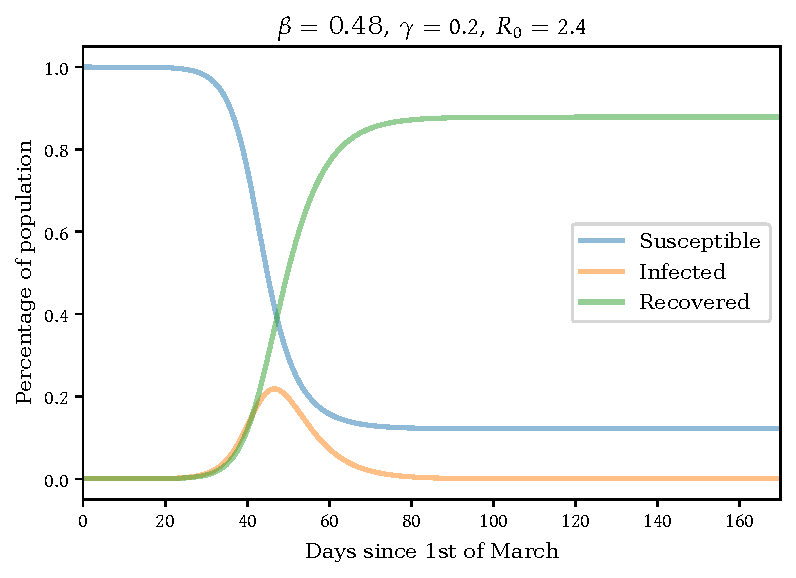
\includegraphics[height=15cm]{sir_example_files/sir_example_8_0.pdf}
    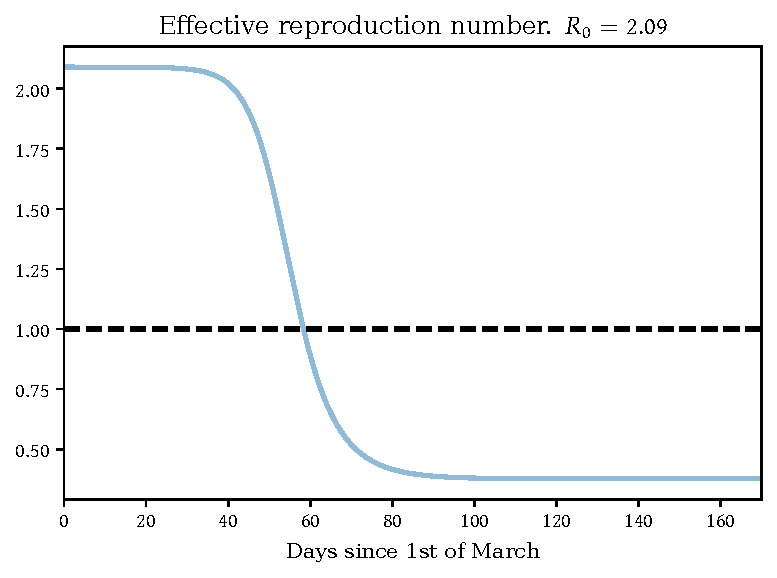
\includegraphics[height=15cm]{sir_example_files/sir_example_20_0.pdf}
  }%
}
\setlength{\twosubht}{\ht\twosubbox}

% typeset

\centering

	\begin{subfigure}[b]{0.48\textwidth}
			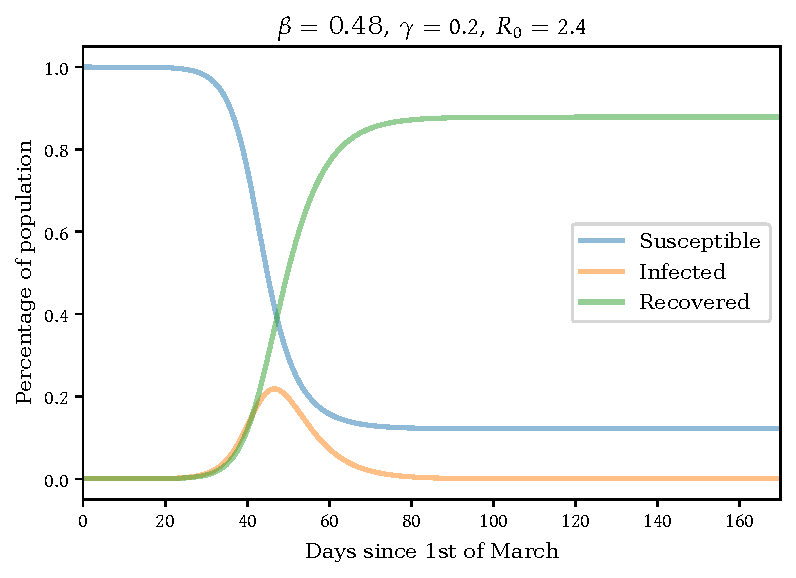
\includegraphics[height = \twosubht]{sir_example_files/sir_example_8_0.pdf}
		\caption{SIR evolution}
		\label{fig:sir_simul_first}
	\end{subfigure}
	\begin{subfigure}[b]{0.48\textwidth}
			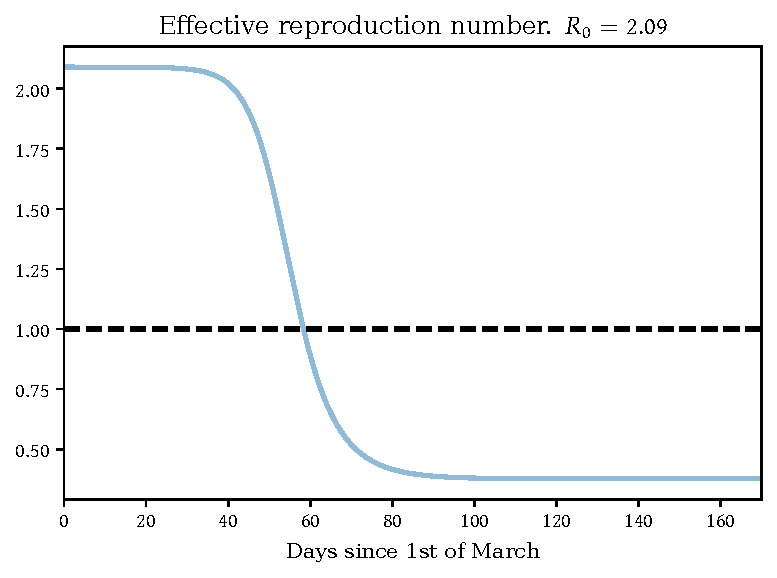
\includegraphics[height = \twosubht]{sir_example_files/sir_example_20_0.pdf}
		\caption{Effective Reproduction Number}
		\label{fig:effective_R0}
	\end{subfigure}
\end{figure}

Our simulation tells us that even with such a high \(\mathcal{R}_0\) the infection dies out relatively quickly. It cannot be distinguished from the figure but our model also predicts a strictly positive share of susceptible people at the end of the sample, which is about \(4\%\) of the population. This is clearly not a really good fit of the data since the estimate used data up to 19th of May. If we update to a more updated estimate of the basic reproduction number to \(\mathcal{R}_0 = 2.09\) and we fix \(\gamma = 0.2\), our \(\beta\) drops to \(0.418\). Which implies that the final amount of susceptible people is much larger at \(18\%\) compared to \(4\%\) before. This shows the extreme importance of reducing the transmission rate, that is why lockdowns and social distancing measures work!

We show in Figure \ref{fig:effective_R0} the behavior of the effective reproduction number over time which is \(\mathcal{R}^e_0 = \mathcal{R}_0 \times S(t)\) which shows that around the 58th day, the effective reproduction number drops to below 1. This coincides with the peak of infected people and not by chance as our model shows!

In this model, initial conditions matter for the peaks as we have seen. If we now drop the initial state for the susceptible population to \(S(0) = 0.6\) and the rest are recovered people, the peak of infections occurs at a much lower rate of only \(2.3\%\) of the population. This shows how new infections would deal in an environment with herd immunity. Dynamics are shown in Figure \ref{fig:sir_simul_S0}. If the amount of immune (recovered) people is sufficiently large, new infections have a much smaller impact. This is what happens with vaccines. If we look at the derived effective reproduction number in Figure \ref{fig:effective_number_S0}, it starts at \(1.25\) and about 30 days later it is at \(1\).

\begin{figure}[htbp]
	% preliminary
	\sbox\twosubbox{%
	  \resizebox{\dimexpr.975\textwidth-1em}{!}{%
		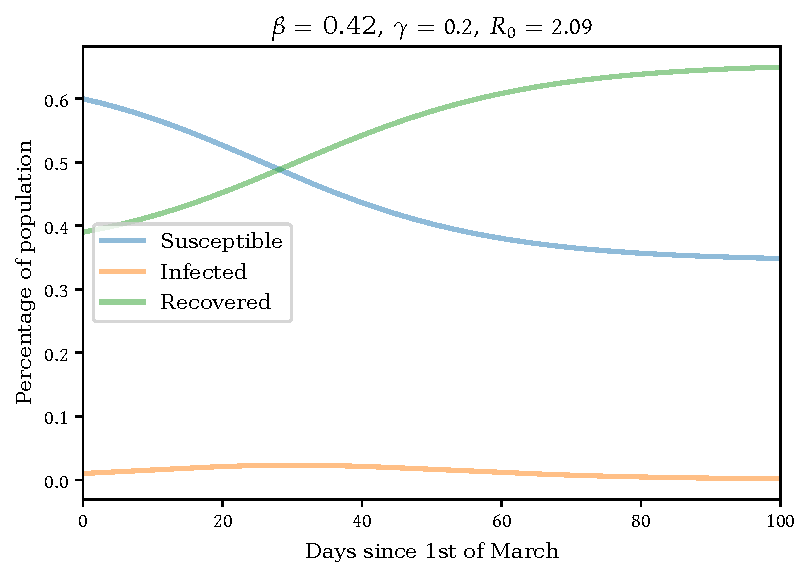
\includegraphics[height=15cm]{sir_example_files/sir_example_11_0.pdf}
		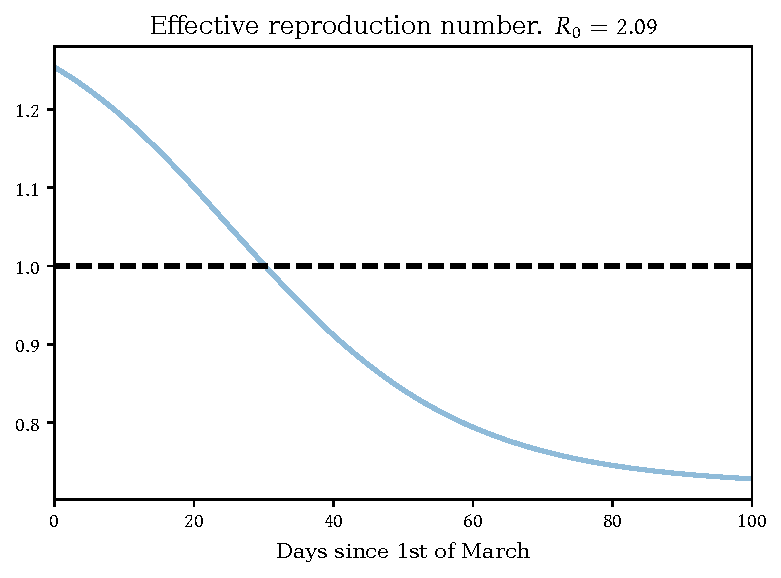
\includegraphics[height=15cm]{sir_example_files/sir_example_13_0.pdf}
	  }%
	}
	\setlength{\twosubht}{\ht\twosubbox}
	
	% typeset
	
	\centering
	
	\begin{subfigure}[b]{0.48\textwidth}
		\centering
			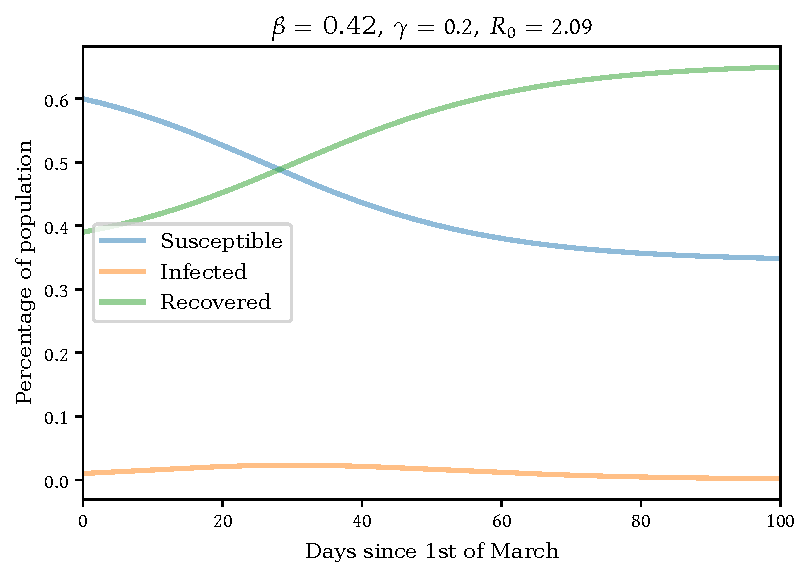
\includegraphics[width = \textwidth]{sir_example_files/sir_example_11_0.pdf}
		\caption{SIR Simulation. Change initial conditions}
		\label{fig:sir_simul_S0}
	\end{subfigure}
	\begin{subfigure}[b]{0.48\textwidth}
		\centering
			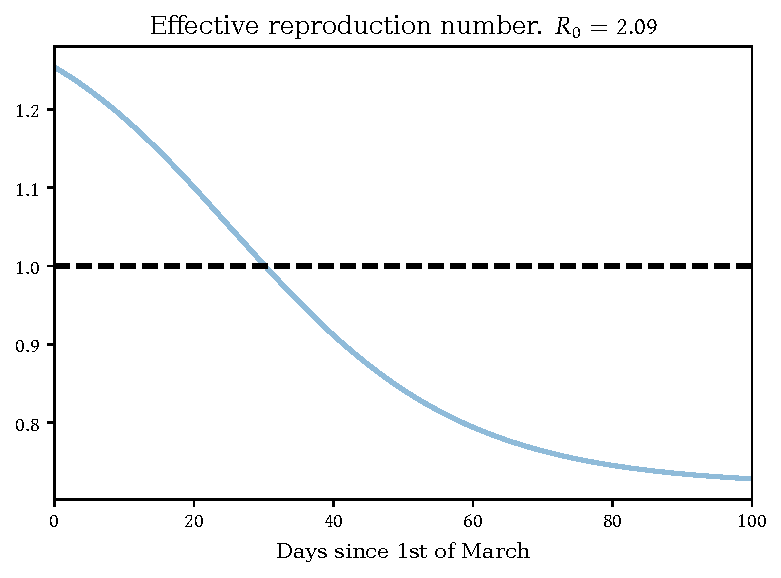
\includegraphics[width = \textwidth]{sir_example_files/sir_example_13_0.pdf}
		\caption{SIR Simulation. Change initial conditions}
		\label{fig:effective_number_S0}
	\end{subfigure}
\end{figure}
    
Clearly, the model has very evident limitations. For starters, we are assuming that the full population gets infected and recovers at the same rate which is against all evidence. Furthermore, our simulations do not incorporate lockdowns nor other policies. We could implement that as shocks to the rate of infection \(\beta\) making it time-dependent \((\beta_t)\). Despite all these limitations, this model helps us understand dynamics that simply from the data cannot be extracted.

The biggest challenges when estimating SIR-type of models is finding the actual moment at which the effective reproduction number drops below one, since that moment determines the peak of infections and influences all the dynamics of the model. Note this is a challenge for several reasons. First, the model is non-linear. Second, the data is very noisy and extremely dependent on the amount of testing, thus testing massively and frequently can help finding out the initial conditions of the system which in fact determine lots of things! Third, it is hard to know which population groups the infection affects the most when the disease is new. Lots of other problems but at least, having a model helps us understand where we have to take action.

\end{document}